% !TEX program = xelatex
\documentclass[tikz, crop, border = {2pt 2pt 2pt 2pt}]{standalone}

\usepackage{concmath-otf}
\usetikzlibrary{calc, angles, quotes, patterns}
\usetikzlibrary{decorations.pathreplacing, decorations.pathmorphing, calligraphy}
\usetikzlibrary{shapes}
\usetikzlibrary{math}

\begin{document}
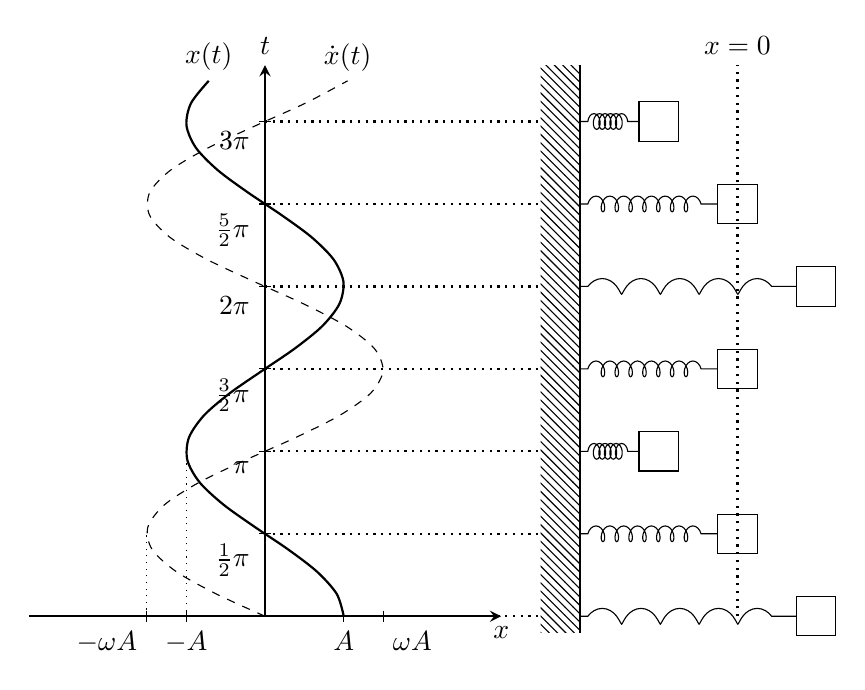
\begin{tikzpicture}

	\tikzmath{
		\amp = 1;
		\omg = 1.5;
	}
	\draw[smooth, domain = 0:6.8, thick] plot ({\amp * cos(\omg*\x r)}, \x) node[above]{$x(t)$}; 
	\draw[smooth, domain = 0:6.8, dashed] plot ({- \amp * \omg * sin(\omg*\x r)}, \x) node[above]{$\dot{x}(t)$};

	\draw (2pt, {1/3 * pi}) -- ++ (-4pt, 0) node[below left]{$\frac{1}{2}\symrm{\pi}$};
	\draw (2pt, {2/3 * pi}) -- ++ (-4pt, 0) node[below left]{$\symrm{\pi}$};
	\draw (2pt, {3/3 * pi}) -- ++ (-4pt, 0) node[below left]{$\frac{3}{2}\symrm{\pi}$};
	\draw (2pt, {4/3 * pi}) -- ++ (-4pt, 0) node[below left]{$2\symrm{\pi}$};
	\draw (2pt, {5/3 * pi}) -- ++ (-4pt, 0) node[below left]{$\frac{5}{2}\symrm{\pi}$};
	\draw (2pt, {6/3 * pi}) -- ++ (-4pt, 0) node[below left]{$3\symrm{\pi}$};

	\draw (\amp, 2pt) -- ++ (0, -4pt) node[below]{$A$};
	\draw (-\amp, 2pt) -- ++ (0, -4pt) node[below]{$-A$};
	\draw[dotted] (-\amp, 2pt) -- ++ (0, {2/3 * pi});
	\draw ({-\omg*\amp}, 2pt) -- ++ (0, -4pt) node[below left]{$-\omega A$};
	\draw ({+\omg*\amp}, 2pt) -- ++ (0, -4pt) node[below right]{$\omega A$};
	\draw[dotted] ({-\omg*\amp}, 0) -- ++ (0, {1/3 * pi});
	
	\begin{scope}[shift = {(6, 0)}]
		\fill[pattern = north west lines] (-2.5, -6pt) rectangle (-2, 7);
		\draw (-2, -6pt) -- (-2, 7);
		\draw[thick, dotted] (0, 0) -- (0, 7) node[above]{$x = 0$};
		\foreach \y in {0, 1, 2, ..., 6} {
			\tikzmath{
				\x = \y / 3;
				\pnt = {\amp * cos(\omg*pi*\x r)};
				\spt = {((\pnt + \amp)^2)*3 + 2};
			}
			\node[draw, rectangle, inner sep = 0.25cm] (a) at (\pnt, {pi*\x}){};

			\draw[decorate, decoration = {coil, amplitude = 0.1cm, segment length = \spt, aspect = 0.6, pre length = 0.1cm, post length = 0.1cm}] (-2, {pi*\x}) -- (a);
			
			\draw[dotted, thick] (-6, {pi*\x}) -- ++ (3.5, 0);
		}
	\end{scope}

	\draw[-stealth, thick] (-3, 0) -- (3, 0) node[below]{$x$};
	\draw[-stealth, thick] (0, 0) -- (0, 7) node[above]{$t$};
\end{tikzpicture}
\end{document}
